\documentclass[12pt]{article}
\usepackage{amsmath, amssymb}
\usepackage{graphicx}
\usepackage{fancyhdr}
\usepackage{enumitem}
\usepackage{multicol}
\usepackage{geometry}
\geometry{margin=1in}

\pagestyle{fancy}
\fancyhf{}
\rhead{MAC 2311 - Calculus I}
\lhead{Exam 1 - Fall 2024}
\cfoot{\thepage}

\begin{document}

\begin{center}
    \textbf{\Large MAC 2311 CALCULUS I --- CRN 85503}\\
    \vspace{0.2cm}
    \textbf{\Large Exam 1}\\
    \vspace{0.2cm}
    Term: Fall, 2024 \\
    \vspace{0.2cm}
    \textbf{Full Name:} \rule{10cm}{0.5pt}
\end{center}

\vspace{0.5cm}

\textbf{Instructions}
\begin{enumerate}[label=\arabic*.]
    \item Total time: 1 hour 15 minutes.
    \item Write the information requested above.
    \item Switch off any electronic devices.
    \item Calculators are not allowed.
    \item Write the solution in the given space.
    \item Show all your work for full credit.
    \item Scratch papers are provided but will not be graded.
    \item You are not allowed to use differentiation rules.
    \item You are not allowed to use L’Hôpital’s Rule in this exam.
\end{enumerate}

\vspace{0.5cm}

\textbf{Formulas}
\begin{itemize}
    \item Slope of a tangent line at \( x = a \) for the curve \( f(x) \): \\
    \[ m = f'(a) = \lim_{x \to a} \frac{f(x) - f(a)}{x - a} \]

    \item Derivative of a function using limit definition: \\
    \[ f'(x) = \lim_{h \to 0} \frac{f(x + h) - f(x)}{h} \]
\end{itemize}

\vspace{0.5cm}

\begin{tabular}{|c|c|c|}
    \hline
    Q.N. & Points & Score \\
    \hline
    1 & 10 & \\
    2 & 10 & \\
    3 & 10 & \\
    4 & 10 & \\
    5 & 10 & \\
    6 & 10 & \\
    7 & 10 & \\
    Bonus & 10 & \\
    \hline
    Total & 70 & \\
    \hline
\end{tabular}

\vspace{1cm}

\begin{enumerate}
    \item (10 points) Find the domain and the inverse of the following functions:
    \begin{enumerate}
        \item \( f(x) = \frac{x^5}{5} - 1 \)
        \item \( y = 3 - \sqrt{x} \)
        \item \( y = \ln(x + 2) \)
    \end{enumerate}

\item (10 points)
\begin{enumerate}
    \item[(a)] (4 pts) Find the equation of the vertical asymptotes \(x = a\) of the function:  
    \[
    f(x) = \frac{x^2 + 2}{x^2 - 7x + 10}
    \]
    \item[(b)] (6 pts)Using the graph of function \( f(x) \) given below, answer the following questions.
        (If a limit does not exist, write “DNE” and if function is undefined at a point, write “undefined”.)
    \begin{figure}[ht!]
        \centering
        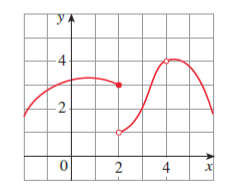
\includegraphics[width=0.35\linewidth]{/Users/melusi/Desktop/Projects/COSC 4315 Project/exam_collection/E1C1Q2b_graph.png}
    \end{figure}

        \begin{enumerate}
            \item \( \lim_{x \to 2^-} f(x) = \)
            \item \( \lim_{x \to 2^+} f(x) = \)
            \item \( \lim_{x \to 2} f(x) = \)
            \item \( f(2) = \)
            \item \( \lim_{x \to 4} f(x) = \)
            \item \( f(4) = \)
        \end{enumerate}
    \end{enumerate}

% Question 3
    \item (10 points)
    \begin{enumerate}
        \item [(a)] (5 pts) Determine the infinite limits:
        \[
        \lim_{x \to 2^+} \frac{x + 1}{x - 2}, \quad 
        \lim_{x \to 4^-} \frac{x}{x - 4}
        \]

        \item [(b)] (5 pts) Find \( f \circ g \circ h \) for the functions: \\
        \( f(x) = 2x + 1,\ g(x) = x^2,\ h(x) = \cos x \)
    \end{enumerate}

% Question 4
    \item (10 points)
    \begin{enumerate}
        \item [(a)]  (5 pts) Solve:
        \[
        x = \log_2 8 + \log_2 \left(\frac{1}{8}\right) + \ln e
        \]

        \item [(b)] (5 pts) Evaluate the limit and find the horizontal asymptotes:
        \[
        \lim_{x \to \infty} \frac{3x^2 - 5x + 2}{4 - 3x - x^2}
        \]
    \end{enumerate}

% Question 5
    \item (10 points) Evaluate the following limits algebraically:
    \begin{enumerate}
        \item [(a)]  \( \lim_{x \to 3} \frac{x^2 - 9}{x^2 - 4x + 3} \)
        \item [(b)] \( \lim_{x \to 0} \frac{(x - 1)^2 - 1}{x} \)
    \end{enumerate}

% Question 6
    \item (10 points) Determine if \( f \) is continuous or discontinuous at the given points. If discontinuous, choose one of: 
    (i) \( f \) is undefined, 
    (ii) limit does not exist, 
    (iii) \( \lim_{x \to a} f(x) \neq f(a) \)

    \begin{figure}[ht!]
        \centering
        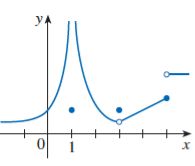
\includegraphics[width=0.35\linewidth]{/Users/melusi/Desktop/Projects/COSC 4315 Project/exam_collection/E1C1Q6_graph.png}
    \end{figure}

    \begin{itemize}
        \item [(a)] At \( x = 1 \)
        \item [(b)] At \( x = 2 \)
        \item [(c)] At \( x = 3 \)
        \item [(d)] At \( x = 4 \)
        \item [(e)] At \( x = 5 \)
    \end{itemize}

 % Question 7
    \item (10 points) Let \( f(x) = x^2 + 3 \)
    \begin{enumerate}
        \item [(a)] Find the derivative \( f'(x) \) using the limit definition.
        \item [(b)] Use \( f'(x) \) to find the slope of the tangent line to the curve at \( x = 1 \).
    \end{enumerate}

% Question 8
    \item[\textbf{Bonus.}] (10 points)
    \begin{enumerate}
        \item Find the value of constant \( c \) so that the function is continuous everywhere:
        \[
        G(x) = 
        \begin{cases}
            4 - \cos x, & x < 0 \\
            \sqrt{x + 3c}, & x \geq 0
        \end{cases}
        \]

        \item Find the horizontal and vertical asymptotes of:
        \[
        f(x) = \frac{2e^x}{e^x - 5}
        \]
    \end{enumerate}
\end{enumerate}

\end{document}
